\documentclass[11pt]{article}


\usepackage[utf8]{inputenc}
\usepackage{tikz}
\usepackage{tikz-3dplot}
\usepackage{tikz-cd}
\usepackage{xcolor}
\usepackage{proof}
\usepackage {alltt}
\usetikzlibrary{shapes.misc}

\usepackage{graphicx} % Allows including images
\usepackage{booktabs} % Allows the use of \toprule, \midrule and \bottomrule in tables
\usepackage{listings}
\usepackage[export]{adjustbox}
\usepackage{verbatim}
\tikzset
  {cross/.style={cross out, draw=black, minimum size=2*(#1-\pgflinewidth), inner sep=0pt, outer sep=0pt},cross/.default={1pt}}

\usetikzlibrary{decorations.markings}
\usepackage{amsmath }
\usepackage{framed}
\usepackage{proof}
\usepackage{enumerate,xspace,stmaryrd}
\usepackage{amsmath,amssymb,latexsym}
\usepackage{textcomp,xspace}
\usepackage[top=2cm, bottom=2.5cm, right=2.5cm, left=2.5cm]{geometry}\usepackage{latexsym}  %For plain TeX symbols, such as \Box used in \qed
\usepackage{euscript}  %%Euler Script font
\usepackage {mdframed}
\usepackage{ifpdf}
\usepackage {alltt}
\renewcommand{\ttdefault}{txtt}
\ifpdf
  \usepackage{epstopdf}
\fi 
\usepackage{etoolbox}
\BeforeBeginEnvironment{tabular}{\begin{center}\small}
\AfterEndEnvironment{tabular}{\end{center}}

\newcommand{\A}{{\ensuremath{\mathbb A}}\xspace}
\newcommand{\B}{{\ensuremath{\mathbb B}}\xspace}
\newcommand{\C}{{\ensuremath{\mathbb C}}\xspace}
\newcommand{\D}{{\ensuremath{\mathbb D}}\xspace}
\newcommand{\F}{{\ensuremath{\mathbb F}}\xspace}
\newcommand{\G}{{\ensuremath{\mathbb G}}\xspace}
\newcommand{\R}{{\ensuremath{\mathbb R}}\xspace}

\newcommand{\rst}[1]{\overline{#1}\,}
\newcommand{\Sets}{{\ensuremath{\sf Sets}}\xspace}
\newcommand{\Cat}{{\ensuremath{\sf Cat}}\xspace}
\newcommand{\llab}[1]{\tiny{\texttt{(+)~~~}}
                      \small{$#1$}
                      \tiny{\texttt{~~~(-)}}
                     }

\newcommand{\spllab}[1]{
                      \texttt{(+)~~~~~~~~~~~~}
                      \small{\texttt{$#1$}}
                      \texttt{~~~~~~~~~~~~(-)}
                     }

\newcommand{\rlab}[1]{\tiny{\texttt{(-)~~~}}
                      \small{$#1$}
                      \tiny{\texttt{~~~(+)}}
                     }

\newcommand{\plab}[1]{\tiny{\texttt{(+)~~~~~}}
                      \small{$#1$}
                     }

\newcommand{\rplab}[1]{
                       \small{$#1$}  
                       \tiny{\texttt{~~~~~(+)}}
                     }

\newcommand{\normlab}[1]{
                       \small{$#1$}  
                     }


\newcommand{\nlab}[1]{\tiny{\texttt{(-)~~~~~}}
                      \small{$#1$}
                     }



\newcommand{\proc}[2] {\small{\sf{$#1$}}\\~~\\ \tiny{{#2}}}

\input xy
\xyoption{all}
\xyoption{2cell}
\UseAllTwocells

\title{Concurrent MPL}

\bibliographystyle{plain}

%%%%%%%%% macros defined %%%%%%%%%%%%%%%%%%%%%%%%%%%%%%%%%%%%%%%%%

\newcommand{\X}{{\ensuremath{\mathbb X}}\xspace}
\newcommand{\Y}{{\ensuremath{\mathbb Y}}\xspace}
\newcommand{\Z}{{\ensuremath{\mathbb Z}}\xspace}

\newcommand{\<}{\langle}
\renewcommand{\>}{\rangle}
\newcommand{\lollipop}{\ensuremath{-\!\!\circ}}

\newcommand{\op}{\ensuremath{^{\textnormal{op}}}}
\renewcommand{\hat}{\widehat}
\renewcommand{\b}{\bullet}
\renewcommand{\c}{\circ}
\newcommand{\ox}{\otimes}         
\newcommand{\x}{\times}     
\newcommand{\fold}[1]{\ensuremath{\left\{\!\!\!\;\left| #1 \right|\!\!\!\;\right\} }}  
\newcommand{\unfold}[1]{\ensuremath{\left(\!\!\!\;\left| #1 \right|\!\!\!\;\right) }}  
\def\endproof{~\hfill$\Box$\vskip 10pt}

\newtheorem{theorem}{Theorem}[section]    
\newtheorem{corollary}[theorem]{Corollary}   
\newtheorem{lemma}[theorem]{Lemma}   
\newtheorem{remark}[theorem]{Remark}   
\newtheorem{example}[theorem]{Example}   
\newtheorem{proposition}[theorem]{Proposition}
\newtheorem{definition}[theorem]{Definition}

\newcommand{\proof}{\noindent{\sc Proof:}\xspace}

\def\monus{\buildrel\textstyle.\over
    {\hbox{\vrule height.55ex width0pt
        \smash{\hbox{\mathsurround=0pt$-$}}}}}
\def\xybox#1#2{\save [].[#2]!C="xb#1"*[F.]\frm{}\restore}


\begin{document}
\maketitle

\section {Concurrent MPL}
For the ease of understanding, MPL programs can be conceptually divided into two levels, namely concurrent MPL programs and sequential MPL programs. In this chapter, various constituents of the concurrent MPL programs are described.
~~\\~~\\ 
Concurrent MPL programs consist of protocols, coprotocols and processes. Protocols and coprotocols are the concurrent analogues of data types and codata types respectively from  sequential MPL. In concurrent MPL, programs are structured using processes. The processes communicate with each other by sending messages over channels. Section \ref {Conc:ChanDesc} describes channels, Section \ref {Conc:ProcDesc} describes processes and Section \ref {Conc:Protcols} describes (co)protocols.
\section {Channels}\label{Conc:ChanDesc}
In message passing view of concurrency, channels are important as they act as the conduit for the exchange of messages between processes. 
~~\\~~\\
Figure \ref {fig:Conc_channels} describes a concurrent MPL program with three processes $\mathbf{P_1}$, $\mathbf{P_2}$ and $\mathbf{P_3}$ represented as circles. A description of the components of the diagram and the relationship between them is below:
\begin {itemize}
  \item $\mathbf{ch1}$ connects process $\mathbf{P_1}$ with process $\mathbf{P_2}$ which is drawn as a solid line between the two processes. Channel $\mathbf{ch1}$ connects the two processes by acting as an output polarity channel for $\mathbf{P_1}$ and an input polarity channel for $\mathbf{P_2}$. The $\texttt{(+)}$ sign on channel $\mathbf{ch1}$ towards $\mathbf{P_1}$ and $\texttt{(-)}$ sign towards $\mathbf{P_2}$ suggests that $\mathbf{ch1}$ acts as an output channel for process $\mathbf{P_1}$ and an input channel for process $\mathbf{P_2}$.
  \item Similarly, $\mathbf{ch2}$ connects processes $\mathbf{P_2}$ and $\mathbf{P_3}$ by acting as an output channel for $\mathbf{P_2}$ and an input channel for $\mathbf{P_3}$.
  \item Normal MPL channels like $\mathbf{ch1}$ and $\mathbf{ch2}$ are attached to a process on its either ends. 
  \item In addition to a normal channel $\mathbf{ch1}$, process $\mathbf{P_1}$ also has a service channel $\mathbf{s1}$. Service channels allow a process to interact with the outside world. For example, using a service channel a process can ask the user to enter an input or it can display its output to the user.
  \item The outside world has been represented through dotted circles in order to differentiate them from normal processes. The service channels have been represented by dotted lines to differentiate them from normal channels.
  \item A noticeable thing about service channels is that they are connected to processes at only one end and not at both the ends like normal channels. Channel $\mathbf{s1}$ acts as an output polarity service channel as suggested by the $\texttt{(+)}$ sign towards process $\mathbf{P_1}$.
  \item Service channels can be of either polarity, output or input. Input polarity service channels have a special name, {\bf console}. 
\end {itemize}

\begin{figure}
\begin{center}
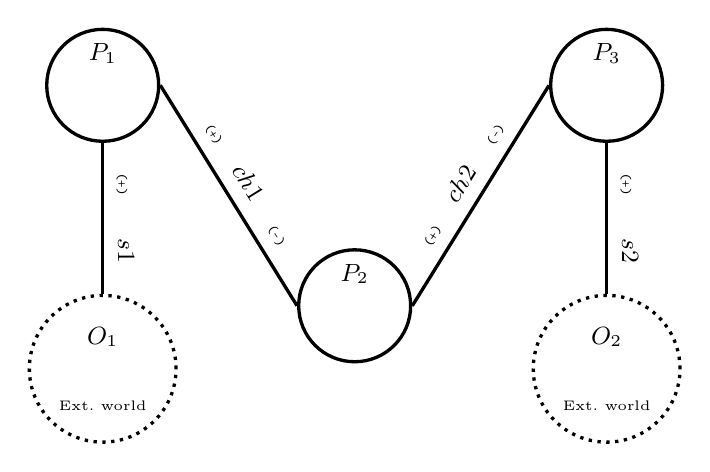
\begin{tikzpicture}[scale = .8,every node/.style={very thick}]
 \draw (0,0)  node[circle,draw=black,minimum size=0.4cm,align=center] (A) 
              {\proc{P_1} {}
              };

 \draw (4,-3.5)  node[circle,draw=black,minimum size=0.4cm,align=center] (B)
              {\proc{P_{2}}{}
              };

 \draw (8,0)  node[circle,draw=black,minimum size=0.4cm,align=center] (C)
              {\proc{P_{3}}{}
              };

 \draw (0,-4.5)  node[circle,draw=black,minimum size=0.4cm,align=center,dotted] (D)
              {\proc{O_{1}}{Ext.~world}
              };

 \draw (8,-4.5)  node[circle,draw=black,minimum size=0.4cm,align=center,dotted] (E)
              {\proc{O_{2}}{Ext.~world}
              };


 \draw[-,draw=black,very thick] (A.east) -- (B.west) 
    node[midway,above=1pt,sloped,fill=white]   {\llab{ch1}};

 \draw[-,draw=black,very thick] (B.east) -- (C.west) 
    node[midway,above=1pt,sloped,fill=white]   {\llab{ch2}};
 
  \draw[-,draw=black,very thick] (A.south) -- (D.north) 
    node[midway,above=1pt,sloped,fill=white]   {\plab{s1}};

  \draw[-,draw=black,very thick] (C.south) -- (E.north) 
    node[midway,above=1pt,sloped,fill=white]   {\plab{s2}};

\end{tikzpicture}
\end{center}
\caption{Processes Connected by Channels} 
\label{fig:Conc_channels}\end{figure}

\section {Processes}\label{Conc:ProcDesc}
Concurrent MPL programs are organised using processes. An example of an MPL process definition has been provided in Figure \ref {fig:Conc_MPLProcs}. A few noticeable things about process definitions in MPL are below:

\begin {itemize}
  \item An MPL process is defined with the keyword {\bf proc} followed by the process name. The process name of the process defined in the example is {\bf someProc}.
  \item An MPL process has sequential and concurrent parameters divided by $\mathbf{\mid}$ sign. Sequential parameters hold the sequential terms are passed to the process when a process call is made. Concurrent parameters are the channels of that process which can be both input and output. \texttt{=>} separates the input polarity channels from the output polarity channels.
  \item In the example, the second line of process definition contains the process parameters, $\texttt{val~|~co~=>~s1}$. $\mathbf{val}$ is the sequential parameter, $\mathbf{co}$ is the input concurrent parameter or the input channel and $\mathbf{s1}$ is the output concurrent parameter or the output channel.  
  \item MPL also allows the programmer to annotate the processes with a type. In the example, the type annotation of $\mathbf{someProc}$ function is present in the first line followed by $\texttt{::}$ symbol. The type of the process is $\texttt{Int |~Console(A) => IntTerm(A)}$ which means that the type of the sequential argument is $\mathbf{Int}$, the type of the input channel is a coprotocol $\mathbf{Console(A)}$ and the type of the output polarity channel is a protocol $\mathbf{IntTerm(A)}$.
  \item The process body is comprised of a sequence of concurrent MPL constructs on the right hand side of $\texttt{->}$. In the example, the process body starts from line 2. Keyword $\mathbf {do}$ is used to define a layout for the the concurrent constructs underneath it, i.e the concurrent constructs can be grouped using alignment and using curly braces is not required. 
  \item A few examples of concurrent MPL constructs are {\sf get, put, id, hput, hcase} etc. Concurrent MPL constructs have been discussed in Section \ref {conc:allConsDesc}.
\end {itemize}

 
\begin{figure}
\begin{alltt}


            proc someProc :: Int | Console (A) => IntTerm (A) = 
                val | co => s1 -> do 
                    hput PutInt on s1 
                    put val on s1
                    hput Close on s1 
                    close s1
                    hput CloseC on co
                    halt co

\end{alltt}
\caption{Example of an MPL Process} 
\label{fig:Conc_MPLProcs}\end{figure}

\section {Protocols/Coprotocols}\label{Conc:Protcols}
An important feature of MPL is that it brings a notion of type safety to the concurrent world. (Co)protocols are central to this notion of type safety. A (co)protocol is the type of a channel. A protocol represents the type of an input channel and a coprotocol represents the type of an output channel. 

\subsection {Achieving Type Safety Using Protocols}
Consider the example of a program in Figure \ref {fig:Conc_TypeSafety} that demonstrates how MPL achieves type safety using protocols. The program has two processes $\mathbf{P_1}$ and $\mathbf{P_2}$ connected via a channel $\mathbf{ch}$. Both the processes try to get a value on the channel $\mathbf{ch}$. {\sf get} is an MPL construct that fetches a value from a channel and {\sf put} is an MPL construct that places a value on a channel. {\sf close} construct closes a channel. 
~~\\~~\\
Intutitively, the configuration in Figure \ref {fig:Conc_TypeSafety} seems wrong because both the processes can't simulatenously get a value on a channel. One process needs to put a value on a channel before another process can read that value from the channel. A configuration like this should result in type error and halt the execution of the program. 
~~\\~~\\
The strategy MPL uses to throw a type error in a configuration like this is to infer the protocols of channel $\mathbf{ch}$ from the two processes it is connecting and check that the two protocols match. If the two protocols don't match a type error is reported.
~~\\~~\\  
Corresponding to every MPL construct, there is an associated base protocol. In order to infer the protocol of channel  $\mathbf{ch}$, consider a few base protocols, {\bf Get}, {\bf Put} and {\bf TopBot}. This is not the exhaustive set of base protocols. The set of all the base protocols have been provided in section \ref {conc:BaseProts}.  
\begin{itemize}
  \item On an output channel, {\sf get} and {\sf put} constructs result in {\bf Get} and {\bf Put} base protocols respectively.
  \item  However, on an input channel,  {\sf get} and {\sf put} constructs result in {\bf Put} and {\bf Get} base protocols respectively. This is done so that the protocols obtained from the processes on the opposite polarities of the channel match.
  \item Closing a channel of any polarity results in the protocol {\bf TopBot}.
\end{itemize}
On inferring the protocol of the channel $\mathbf{ch}$ from processes $\mathbf{P_1}$ and $\mathbf{P_2}$, $\mathbf {Get(A \mid TopBot)}$ and $\mathbf {Put(A \mid TopBot)}$ are obtained respectively. Since, the two protocols don't agree, a type error in thrown halting the execution of the program.
\begin{figure}
\begin{center}
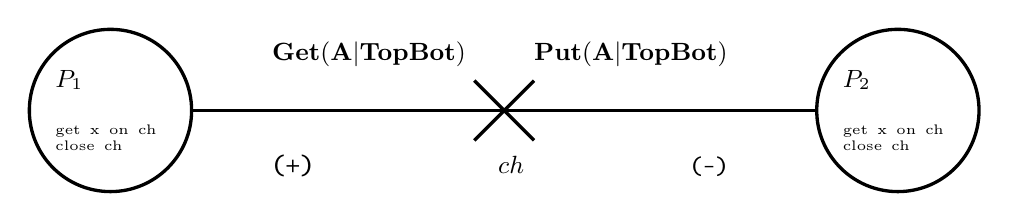
\begin{tikzpicture}[scale = 2,every node/.style={very thick}]
 \draw (0,0)  node[circle,draw=black,text width = 1.4cm,align=left] (A) 
              {\proc{P_1}{
                           get~x~on~ch \\
                           close~ch \\ 
                         }
              };

 \draw (5,0)  node[circle,draw=black,text width = 1.4cm,align=left] (B)
              {\proc{P_2}{
                           get~x~on~ch \\
                           close~ch\\
                         }
              };

\draw (2.5,0) node[cross = 12 pt,very thick,black] {};

\draw[-,draw=black,very thick] (A.east) -- (B.west) 
    node[midway,above=12pt,sloped,fill=white] 
      {\normlab{\mathbf{Get(A|TopBot)~~~~~~~~Put(A|TopBot)}} 
      };
\draw[-,draw=black,very thick] (A.east) -- (B.west) 
    node[midway,below=12pt,sloped,fill=white] 
      {\spllab {ch} 
      };
\end{tikzpicture}
\end{center}
\caption{Example of an MPL Process} 
\label{fig:Conc_TypeSafety}
\end{figure}

\subsection {Base Protocols}\label{conc:BaseProts}
All the (co)protocols in MPL are constructed using the following base protocols. 
\begin{itemize}
  \item Get
  \item Put
  \item $\otimes$ (Tensor)
  \item $\oplus$ (Par)
  \item TopBot
\end{itemize}

\subsection {Defining (Co)Protocols in MPL}
MPL allows the programmers to define complex (co)protocols using base protocols. An example of user defined (co)protocol definitions can be seen in Figure \ref {fig:Conc_ProtDefn}. A few observations about the protocol definition are below:
\begin{itemize}
  \item A protocol is defined using the keyword {\bf protocol}.
  \item The name of the defined protocol in the example is {\bf IntTerm}. This protocol is polymorphic in type variable $\mathbf{A}$.
  \item The syntax $\texttt{IntTerm(A) => P}$ is inspired by the syntax of a data type. In data type definition this syntax is used to convey that a data type is an initial algebra. Here, the same syntax has been used to suggest that protocols are data types of the concurrent world. Very naively, $\mathbf{P}$ can be thought as a synonym or a place holder for $\mathbf{IntTerm(A)}$.
  \item Protocol $\mathbf {IntTerm}$ has three constructors, $\mathbf {GetInt}$, $\mathbf {PutInt}$ and $\mathbf {Close}$. In concurrent MPL, these constructors are known as handles.
  \item If the type of a channel is $\mathbf {IntTerm}$ then it means that any of the three handles of $\mathbf {IntTerm}$ can be put on the channel. Once a handle has been put on a channel, the only actions allowed on the channel are the actions permitted by the protocols of that handle.
  \item $\mathbf{GetInt}$ and $\mathbf{PutInt}$ handles are recursive.
\end{itemize}
Coprotocols are the codata types of the concurrent world and its syntax tries to mimick the syntax of codata types. Coprotocols are associated with the input channels. The destructors of the coprotocols are known as cohandles in concurrent MPL.

\begin{figure}
\begin{alltt}
                protocol IntTerm (A) => P = 
                      GetInt :: Get (A|P) => P
                      PutInt :: Put (A|P) => P
                      Close  :: TopBot    => P

                coprotocol CP => Console (A) =
                    GetIntC   :: CP => Put (A|CP)  
                    PutIntC   :: CP => Get (A|CP) 
                    CloseC    :: CP => TopBot  
\end{alltt}
\caption{(Co)Protocol Definition in MPL} 
\label{fig:Conc_ProtDefn}
\end{figure}


\section {Concurrent MPL constructs}\label{conc:allConsDesc}
Concurrent MPL constructs are the constructs using which concurrent MPL programs are written. They are {\sf plug}, {\sf id}, {\sf hput-hcase}, {\sf get-put}, {\sf split-fork} and {\sf close-halt}. A few noticeable observations about concurrent MPL constructs are below:
\begin{itemize}
  \item MPL constructs with the exception of the {\sf run} contruct perform an action on a channel. In MPL concurrency is modeled using message passing between processes and channels are the conduit through which the messages are exchanged. So, it is only logical that most constructs deal with channel.
  \item Most concurrent MPL constructs come in pair, i.e {\sf get-put}, {\sf hput-hcase}, {\sf split-fork} and {\sf halt-close}. {\sf id}, {\sf run} and {\sf plug} are standalone constructs. The constructs of the pair are dual to each other.
  This is intuitive because in message passing view of concurrency for a process to respond to an action, another process should drive that action on the opposite end of the channel and viceversa. Thus one of the constructs in any pair of constructs is a driver construct and the other is a reaction construct. For example, for a process to get a value on a channel, some other process should have put a value on the channel. Thus, {\sf get} is a reaction construct driven by {\sf put} construct.
\end{itemize}
A brief description of all the concurrent MPL constructs has been provided in Table \ref {Conc:constr_desc}. In the next few sections (Section \ref {conc:run_desc} to Section \ref {conc:haltclosedesc}), various concurrent MPL constructs are described in details.

\begin{table}
\begin{center}
    \begin{tabular}{|l||l|}
    \hline 
        {\sf run} & calls a process \\ \hline 
        {\sf id}  & equates two channels \\ \hline 
        {\sf plug} & connects two processes by a channel \\ \hline  
        {\sf get} & gets a value on a channel \\ \hline 
        {\sf put} & puts a value on a channel \\ \hline 
        {\sf hput} & puts a handle on a channel \\ \hline 
        {\sf hcase} & cases on the handles obtained on channel \\ \hline 
        {\sf split} & splits a channel into two channels \\ \hline 
        {\sf fork} & forks two new processes \\ \hline 
        {\sf close} & closes a channel \\ \hline 
        {\sf halt} & closes a channel. Usually the last channel is halted. \\ \hline
   \end{tabular}
\caption{Machine Transitions for the SAMPL}
\label{Conc:constr_desc}
\end{center}
\end{table}


\subsection{run Construct}\label{conc:run_desc}
{\sf run} construct is used to call an already defined process. This can be thought of as the concurrent counterpart of a function call. To successfully {\sf run} (call) a process from other processes, :
\begin{itemize}
  \item the process being called should already be defined and
  \item the process call should happen with appropriate arguments, i.e the number and type of the process arguments in {\sf run} should be the same as the number and type of the parameters in the process definition.
\end {itemize}
\subsubsection {run Example} 

Table \ref {Conc : runExample} shows an example of an MPL program where {\sf run} construct is used. The output of the program is integer 5 printed on its output service channel, intTerm1. Notesworthy facts about the program are below:

\begin{itemize}
  \item Program defines a recursive protocol, IntTerm and a recursive coprotocol, Console for the input and output service channels respectively.

  \item Inside the main process, process {\bf p1} is {\sf run} (called) with 3 arguments, one sequential and two concurrent. The sequential argument in the process call is the integer value {\bf 5}. Concurrent arguments of a process call are the channels of that process. $\texttt{=>}$ separates concurrent input arguments (input channels) from concurrent output arguments (output channels). The concurrent input argument in the example is the service channel console and the concurrent output argument is the service channel intTerm1. 
  \item The process definition for $\mathbf{p1}$ has 1 sequential parameter, 1 input concurrent parameter and 1 output concurrent parameter. Thus the process call is consistent with the process definition with respect to the number of arguments of each type. 
\end{itemize}
\begin{table}
\begin{center}
\begin{tabular}{|c|} \hline
\begin{minipage}{5in}
{
\begin{alltt}


    protocol IntTerm (A) => P =
        GetInt    :: Get (A|P) => P 
        PutInt    :: Put (A|P) => P
        Close     :: TopBot    => P  

    coprotocol CP => Console (A) =
        GetIntC   :: CP => Put (A|CP)  
        PutIntC   :: CP => Get (A|CP) 
        CloseC    :: CP => TopBot 

    proc p1 :: Int | Console (A) => IntTerm (A) = 
        val | co => s1 -> do 
            hput PutInt on s1 
            put val on s1
            hput Close on s1 
            close s1
            hput CloseC on co
            halt co

    run => intTerm2 -> do 
          p1 ( 5 | console => intTerm1 )

\end{alltt}

} 
\end {minipage} 
\tabularnewline
\hline
\end{tabular}
\caption{Example : {\sf run} construct}
\label{Conc : runExample}
\end{center}
\end{table}



\subsection{plug Construct}
{\sf plug} command connects two processes via a channel. Once the two processes are connected, they can exchange messages. Syntax of plug is shown below:
    \begin{alltt}
              plug
                  p1 ( | console => ch)
                  p2 ( | ch => intTerm1)
    \end{alltt} 
Syntax consists of the keyword {\sf plug} along with the processes being plugged. For a channel to be successfully plugged between two processes, 
\begin{itemize}
  \item it should act as an output channel for one process and an input channel for the other process, and
  \item the protocol of the channel inferred from both the processes it is plugged between should be the same.
\end{itemize}
One can plug multiple processes using the {\sf plug} construct as can be seen below where $\mathbf{ch1}$ is plugged between $\mathbf{p1}$ and $\mathbf{p2}$ and  $\mathbf{ch2}$ is plugged between $\mathbf{p2}$ and $\mathbf{p3}$.

    \begin{alltt}
              plug
                  p1 ( | console => ch1)
                  p2 ( | ch1 => ch2)
                  p3 ( | ch2 => intTerm1)
    \end{alltt}

\subsection {get-put Constructs}
These are the simplest MPL constructs. {\sf get} receives a value on a channel and {\sf put} puts a value on a channel. 
\begin{itemize}
  \item On an output channel, {\sf get} results in {\bf Get} protocol and {\sf put} results in {\bf Put} protocol.
  \item On an input channel, {\sf get} and {\sf put} constructs result in {\bf Put} and {\bf Get} protocols respectively.
\end{itemize}
Thus, {\sf get/put} constructs result in different protocols depending on the polarity of the channel over which they act. This is done in order to infer the same protocol for a channel from the two processes attached at the two ends of the channel.

\subsubsection {get-put Example}
Table \ref {Conc : getputExample} shows an example of an MPL program that uses {\sf get-put} construct. Figure \ref {fig:Conc_getput} shows the diagrammatic representation for the example program in Table \ref {Conc : getputExample}.
~~\\~~\\ 
In the program there are three processes, $\mathbf {p1}$, $\mathbf {p2}$ and $\mathbf {p3}$ apart from the main process. These processes have been represented by three circles named as $\mathbf{P_1}$, $\mathbf{P_2}$ and $\mathbf {P_3}$ respectively in the diagram.
~~\\~~\\
Channel $\mathbf {ch2}$ is plugged between processes $\mathbf {p2}$ and $\mathbf {p3}$ and channel $\mathbf {ch1}$ is plugged between processes $\mathbf {p3}$ and $\mathbf {p1}$. $\mathbf {ch2}$ acts as an output channel for process $\mathbf {p2}$ and an input channel for process $\mathbf {p3}$. The $\mathbf {\texttt{(+)}}$ sign on $\mathbf {ch2}$ at process $\mathbf {P_2}$'s end signifies that $\mathbf {ch2}$ acts as an output channel for process $\mathbf {P_2}$. The $\mathbf {\texttt{(-)}}$ sign on $\mathbf {ch2}$ at process $\mathbf {P_3}$'s end signifies that $\mathbf {ch2}$ acts as an input channel for process $\mathbf {P_3}$. Both $\mathbf {P_2}$ and $\mathbf {P_1}$ have an output service channel named $\mathbf {S1}$ and $\mathbf {S2}$ respectively.
~~\\~~\\ 
When the program is executed, a terminal (service channel intTerm1) pops up asking for a value to be entered. Once the user has entered a value, another terminal (service channel intTerm2) pops up displaying this value.
~~\\~~\\ 
Process $\mathbf {P_2}$ asks for a value on its service channel $\mathbf {S1}$ after putting the appropriate handle on the channel. $\mathbf {P_2}$ then puts this value on its output channel $\mathbf {ch2}$.
~~\\~~\\
Process $\mathbf {P_3}$ reads the value on channel $\mathbf {ch2}$ which is an input channel for $\mathbf {P_3}$. $\mathbf {P_3}$ then puts this value on its output channel $\mathbf {ch1}$.
~~\\~~\\ 
Process $\mathbf {P_1}$ reads the value on channel $\mathbf {ch1}$ which is an input channel for $\mathbf {P_1}$. $\mathbf {P_1}$ then puts this value on service channel $\mathbf {S2}$ after putting the appropriate handle. This value is now visible to the outside world.

\begin{table}
\begin{center}
\begin{tabular}{|c|} \hline
\begin{minipage}{5in}
{
\begin{alltt}


    protocol IntTerm (A) => P =
        GetInt    :: Get (A|P) => P 
        PutInt    :: Put (A|P) => P
        Close     :: TopBot    => P  


    proc p2 :: |  => IntTerm (Int),Put(Int|TopBot) =
        |  => s1,ch2 -> do 
            hput GetInt on s1
            get x on s1
            put x on ch2
            hput Close on s1
            close s1 
            halt ch2


    proc p3 :: |  Put (Int|TopBot) => Put (Int|TopBot) =
        | ch2 => ch1 -> do 
           get x on ch2
           put x on ch1 
           close ch2
           halt ch1

    proc p1 :: | Put (Int|TopBot) => IntTerm (Int) = 
         | ch1 => s2 -> do 
            get x on ch1 
            hput PutInt on s2 
            put x on s2 
            hput Close on s2 
            close s2
            halt ch1

    run => intTerm1,intTerm2 -> do 
        plug
          p2 ( | => intTerm1,ch2)  
          p3 ( | ch2 => ch1) 
          p1 ( | ch1 => intTerm2 )



\end{alltt}

} 
\end {minipage} 
\tabularnewline
\hline
\end{tabular}
\caption{Example : {\sf get-put} constructs}
\label{Conc : getputExample}
\end{center}
\end{table}


\begin{figure}
\begin{center}
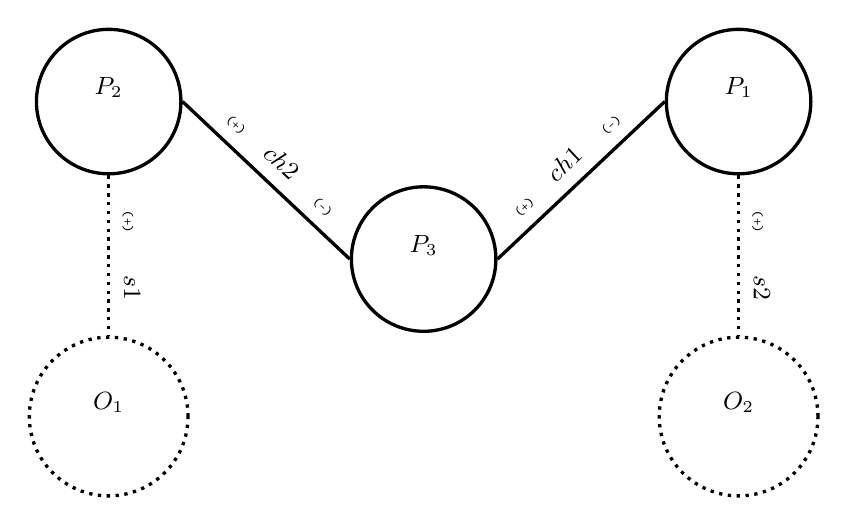
\begin{tikzpicture}[ scale = 2,
                     every node/.style={very thick},draw = black,
                   ]
 \draw (0,0)  node[circle,draw=black,text width = 1.4cm,align=center] (A) 
              {\proc{P_2}{ 
                         }
              };

 \draw (4,0)  node[circle,draw=black,text width = 1.4cm,align=center] (B)
              {\proc{P_1}{ 
                         }
              };

 \draw (4,-2) node[circle,draw = black,text width = 1.6cm,align=center,dotted] (D)
              {\proc{O_2}{}
              };

 \draw (0,-2) node[circle,draw=black,text width = 1.6cm,align=center,dotted] (E)
              {\proc{O_1}{}
              };

 \draw (2,-1) node[circle,draw=black,text width = 1.4cm,align=center] (C) 
              {\proc{P_3}{
                         }
              };

 \draw[-,draw=black,very thick] (A.east) -- (C.west) 
    node[midway,above=1pt,sloped,fill=white]   {\llab{ch2}};
 \draw[-,draw=black,very thick] (C.east) -- (B.west) 
    node[midway,above=1pt,sloped,fill=white]   {\llab{ch1}};
 \draw[-,draw=black,very thick,dotted] (B.south) -- (D.north) 
    node[midway,above=1pt,sloped,fill=white]   {\plab{s2}};
 \draw[-,draw=black,very thick,dotted] (A.south) -- (E.north) 
    node[midway,above=1pt,sloped,fill=white]   {\plab{s1}};

\end{tikzpicture}
\end {center}
\caption{{\sf get-put} Example} 
\label{fig:Conc_getput}\end{figure}

\subsubsection {Concurrency Semantics and get Before put}
The program in Table \ref {Conc : getputExample} is simple to understand if one considers that the the processes are scheduled and executed in the order $\mathbf {P_2}$, $\mathbf {P_3}$, and $\mathbf {P_1}$. i.e, $\mathbf {P_2}$ gets a value and passes it to $\mathbf {P_3}$ which in turn passes to $\mathbf {P_1}$. However, the concurrency semantics for MPL allows the processes to be scheduled in any order. For example - order $\mathbf {P_1}$, $\mathbf {P_2}$, and $\mathbf {P_3}$ is also a valid schedule of the processes. The problem with the second schedule is that process $\mathbf {P_1}$ is requesting a get on its input channel $\mathbf {ch1}$ even before process $\mathbf {P_3}$ had the opportunity to put the value on that channel. Similarly, process $\mathbf {P_3}$ is trying to get a value on channel $\mathbf {ch2}$ even before $\mathbf {P_2}$ puts a value on $\mathbf {ch2}$. 
~~\\~~\\ 
MPL handles the above mentioned scenario of trying to get a value before put has happened by putting the process requesting the get operation to sleep and removing it from the set of active processes. Once the value has been put on the channel, the process requesting get is worken up and put in the set of active processes from where it can scheduled. This mechanism is used not only with {\sf get-put} but also with other concurrent construct pairs like {\sf split-fork} and {\sf hput-hcase}, when the process containing the reaction construct of the pair is scheduled before the process containing the driver construct.
\subsection {id Construct}
{\sf id} construct equates two channels. Syntax $\mathbf {\texttt{ch2~|=|~ch1}}$ means that channel $\mathbf{ch1}$ has been equated with channel $\mathbf{ch2}$ meaning:

\begin{itemize}
  \item messages written on $\mathbf{ch1}$ are now available on $\mathbf{ch2}$, i.e one can read messages available on $\mathbf{ch1}$ using $\mathbf{ch2}$, and
  \item messages to be sent via $\mathbf{ch1}$ can now be sent via $\mathbf{ch2}$, i.e. one can write a message on $\mathbf{ch2}$ such that it can be read on $\mathbf{ch1}$.
\end{itemize}

\subsubsection {id Example}

Table \ref {Conc : idExample} represents an example of a program using the {\sf id} construct. The process connectivity diagram for the program has been shown in Figure \ref {fig:Conc_id_exam}.
~~\\~~\\
Process $\mathbf{P_1}$ has an input polarity service channel $\mathbf{s1}$ and an output channel $\mathbf{ch1}$. Process $\mathbf{P_2}$ has an input channel $\mathbf{ch1}$ and an output channel $\mathbf{ch2}$. Process $\mathbf{P_2}$ equates channel $\mathbf{ch1}$ with channel $\mathbf{ch2}$. Process $\mathbf{P_3}$ has an input channel $\mathbf{ch2}$ and an output polarity service channel $\mathbf{s2}$.
~~\\~~\\ 
Process $\mathbf{P_1}$ gets a value from outside world on $\mathbf{s1}$ and puts this value on $\mathbf{ch1}$. Since, $\mathbf{ch1}$ and $\mathbf{ch2}$ have been equated, the value put on $\mathbf{ch1}$ is available on $\mathbf{ch2}$ which is read by process $\mathbf{P_3}$. $\mathbf{P_3}$ subsequently puts the value obtained on $\mathbf{ch2}$ on its service channel $\mathbf{s2}$.
Similarly, process $\mathbf{P_3}$ reads a value on channel $\mathbf{s2}$ which is received by $\mathbf{P_1}$ via process $\mathbf{P_2}$. $\mathbf{P_1}$ then outputs the received value on its service channel $\mathbf{s1}$.

\begin{table}
\begin{center}
\begin{tabular}{|c|} \hline
\begin{minipage}{5in}
{
\begin{alltt}


      coprotocol CP => Console (A) =
          GetIntC   :: CP => Put (A|CP)  
          PutIntC   :: CP => Get (A|CP) 
          CloseC    :: CP => TopBot  

      protocol IntTerm (A) => P =
          GetInt   :: Get (A|P) => P 
          PutInt   :: Put (A|P) => P
          Close    :: TopBot    => P  

      proc p1 = 
        | s1 => w1 -> do 
             hput GetIntC on s1
             get val on s1
             put val on w1
             get val2 on w1
             hput PutIntC on s1
             put val2 on s1 
             close w1
             hput CloseC on s1
             halt s1

      proc p2 =
        | w1 => w2 -> do 
             w2 |=| w1 

      proc  p3 =
          | w2 => s2 -> do 
             get val on w2 
             hput PutInt on s2
             put val on s2
             hput GetInt on s2
             get val2 on s2
             put val2 on w2
             hput Close on s2
             close s2
             halt w2  


      run console => intTerm1 -> do 
          plug 
            p1 ( | console => w1)
            p2 ( | w1 => w2)
            p3 ( | w2 => intTerm1) 


\end{alltt}

} 
\end {minipage} 
\tabularnewline
\hline
\end{tabular}
\caption{Example : {\sf id} construct}
\label{Conc : idExample}
\end{center}
\end{table}

\begin{figure}
\begin{center}
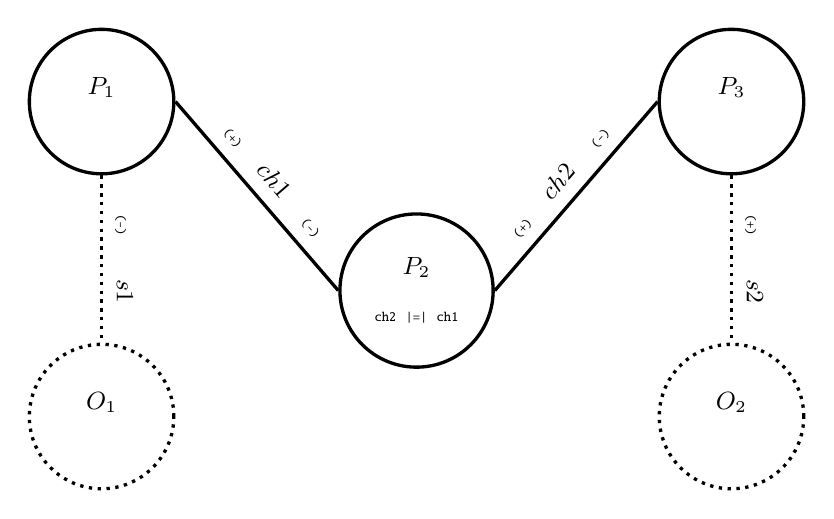
\begin{tikzpicture}[scale = 2,every node/.style={very thick}]
 \draw (0,0)  node[circle,draw=black,text width = 1.4cm,align=center] (A) 
              {\proc{P_1}{

                         }
              };


 \draw (4,0)  node[circle,draw=black,text width = 1.4cm,align=center] (B)
              {\proc{P_3}{


                         }
              };

 \draw (4,-2) node[circle,draw=black,text width = 1.4cm,align=center,dotted] (D)
              {\proc{O_2}{}
              };

 \draw (0,-2) node[circle,draw=black,text width = 1.4cm,align=center,dotted] (E)
              {\proc{O_1}{}
              };

 \draw (2,-1.2) node[circle,draw=black,text width = 1.4cm,align=center] (C) 
              {\proc{P_2}{
                           $\texttt{ch2 |=| ch1}$\\
                         }
              };

 \draw[-,draw=black,very thick] (A.east) -- (C.west) 
    node[midway,above=1pt,sloped,fill=white]   {\llab{ch1}};
 \draw[-,draw=black,very thick] (C.east) -- (B.west) 
    node[midway,above=1pt,sloped,fill=white]   {\llab{ch2}};
 \draw[-,draw=black,very thick,dotted] (B.south) -- (D.north) 
    node[midway,above=1pt,sloped,fill=white]   {\plab{s2}};
 \draw[-,draw=black,very thick,dotted] (A.south) -- (E.north) 
    node[midway,above=1pt,sloped,fill=white]   {\nlab{s1}};

\end{tikzpicture}
\end {center}
\caption{{\sf id} Example} 
\label{fig:Conc_id_exam}
\end{figure}

\subsection {hput-hcase Constructs}

{\sf hput} puts a (co)handle of a (co)protocol on a channel. A handle is {\sf hput} on a channel at one end and {\sf hcased} at the other end. {\sf hcase} can be thought of as concurrent counter part of the {\sf case} construct from the sequential MPL. {\sf case} branches on the constructors of a data type and executes a sequential construct corresponding to the data constructor selected from the branch. {\sf hcase} branches on the handles of a protocol and run a sequence of concurrent commands corresponding to the selected handle from the branch.
~~\\~~\\
One {\sf hputs} a handle on an output channel and {\sf hcases} on handles on an input channel. Conversely, one {\sf hputs} a cohandle on an input channel and {\sf hcases} on cohandles on an output channel.

\subsubsection {hput-hcase Example}
Table \ref {Conc : hcaseExample} shows an example of a program that uses the {\sf hput-hcase} constructs. The process connectivity diagram for the program has been shown in Figure \ref {fig:Conc_hcase_exam}.
~~\\~~\\ 
Process $\mathbf{P_1}$ has an output service channel $\mathbf{i1}$ and a normal output channel $\mathbf{ch}$. Process $\mathbf{P_2}$ has an output service channel $\mathbf{i2}$ and a normal input channel $\mathbf{ch}$. $\mathbf{ch}$ has been plugged between processes $\mathbf{P_1}$ and $\mathbf{P_2}$.
~~\\~~\\ 
Process $\mathbf{P_1}$ performs the following actions in sequence:
\begin{itemize}
  \item It reads an integer value on $\mathbf{i1}$
  \item It hputs a handle $\mathbf {PutInt}$ on channel $\mathbf{ch}$ indicating that it plans to put a value on the channel. 
  \item It puts the value read from on $\mathbf{i1}$ on the channel $\mathbf{ch}$. 
  \item It hputs a handle $\mathbf {GetInt}$ on channel $\mathbf{ch}$ indicating that it expects to receive a value on the channel. 
  \item It receives a value on the channel $\mathbf{ch}$ and then puts this value on $\mathbf{i1}$. 
\end{itemize}
Process $\mathbf{P_2}$ hcases on the handle obtained on channel $\mathbf{ch}$ and performs the following actions for the below handles:
\begin{itemize}
  \item {\bf GetInt} : Corresponding to this handle, the process reads value from its service channel $\mathbf{i2}$ and puts it on channel $\mathbf{ch}$.
  \item {\bf PutInt} : Corresponding to this handle, the process reads a value from channel $\mathbf{ch}$ and puts it on $\mathbf{i2}$.
  \item {\bf Close}  : Corresponding to this handle, the channels are closed and the process is terminated.
\end{itemize}
The final output is a terminal that pops up and asks for a integer value. Once the value is entered, another terminal pops up and displays the value entered on the first terminal. The second terminal then asks for a value which is displayed in the first terminal. The popping terminals are the service channels.

\begin{table}
\begin{center}
\begin{tabular}{|c|} \hline
\begin{minipage}{3.2in}
{
\begin{alltt}

oprotocol CP => Console (A) =
    GetIntC   :: CP => Put (A|CP)  
    PutIntC   :: CP => Get (A|CP) 
    CloseC    :: CP => TopBot  

protocol IntTerm (A) => P =
    GetInt   :: Get (A|P) => P 
    PutInt   :: Put (A|P) => P
    Close    :: TopBot    => P  

proc p1 = 
    | co => i1,ch -> do 
        hput GetInt on i1 
        get x on i1 
        hput PutInt on ch 
        put x on ch 
        hput GetInt on ch 
        get y on ch 
        hput PutInt on i1 
        put y on i1 
        hput Close on i1 
        close i1 
        hput Close on ch 
        close ch 
        hput CloseC on co 
        halt co 

proc p2 = 
    | ch => i2 -> 
        hcase ch of 
            GetInt -> do 
                hput GetInt on i2  
                get x on i2 
                put x on ch 
                p2 ( | ch => i2)

            PutInt -> do 
                get x on ch 
                hput PutInt on i2 
                put x on i2
                p2 ( | ch => i2)

            Close  -> do 
                hput Close on i2 
                close i2
                halt ch 

run console => intTerm1,intTerm2 -> 
      plug 
         p1 ( | console => ch,intTerm1)
         p2 ( | ch => intTerm2)
 
\end{alltt}

} 
\end {minipage} 
\tabularnewline
\hline
\end{tabular}
\caption{Example : {\sf hput-hcase} constructs}
\label{Conc : hcaseExample}
\end{center}
\end{table}

\begin{figure}
\begin{center}
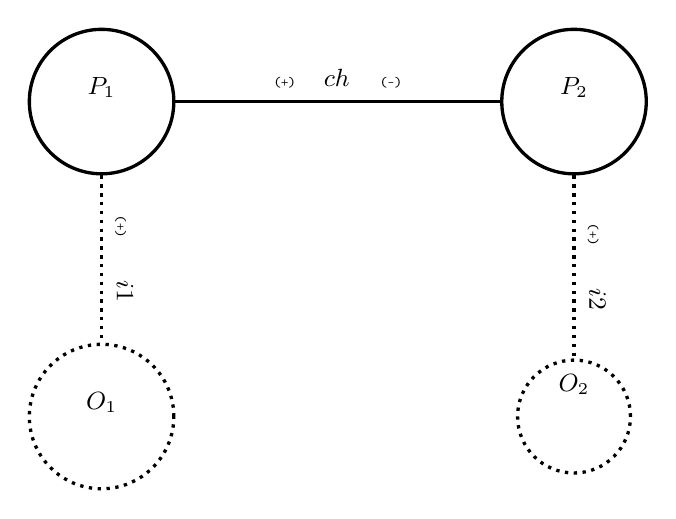
\begin{tikzpicture}[scale = 2,every node/.style={very thick}]
 \draw (0,0)  node[circle,draw=black,text width = 1.4cm,align=center] (A) 
              {\proc{P_1}{

                         }
              };


 \draw (3,0)  node[circle,draw=black,text width = 1.4cm,align=center] (B)
              {\proc{P_2}{


                         }
              };

 \draw (3,-2) node[circle,draw=black,align=center,dotted] (D)
              {\proc{O_2}{}
              };

 \draw (0,-2) node[circle,draw=black,text width = 1.4cm,align=center,dotted] (E)
              {\proc{O_1}{}
              };

 \draw[-,draw=black,very thick] (A.east) -- (B.west) 
    node[midway,above=1pt,sloped,fill=white]   {\llab{ch}};

 \draw[-,draw=black,very thick,dotted] (B.south) -- (D.north) 
    node[midway,above=1pt,sloped,fill=white]   {\plab{i2}};
 \draw[-,draw=black,very thick,dotted] (A.south) -- (E.north) 
    node[midway,above=1pt,sloped,fill=white]   {\plab{i1}};

\end{tikzpicture}
\end {center}
\caption{{\sf hput-hcase} Example} 
\label{fig:Conc_hcase_exam}
\end{figure}

\subsection {split-fork Constructs}
Creating/forking new processes is a natural requirement in many concurrent programs. In MPL, creation of new processes is achieved using the {\sf fork} construct that creates two new processes from an old process. In MPL processes are usually connected to other processes via channeels. However, after forking both the newly forked processes need their own channel to maintain the connectivity that the parent process had with the other processes. {\sf split} takes a channel and divides it into two channels. 
~~\\~~\\ 
{\sf split} and {\sf fork} are dual to each other. Splitting an input channel or forking on an output channel results in the protocol $\mathbf {\otimes}$ (tensor). Splitting an output channel or forking on an input channel results in the protocol $\mathbf {\oplus}$ (par).

\subsubsection {split-fork Example}

Table \ref {Conc : sForkExample} shows an example of a program that uses the {\sf split-fork} constructs. The configuration of the processes before and after the {\sf split-fork} occurs is shown through the two diagrams in Figure \ref {fig:Conc_sfork_exam}. The first diagram shows the before configuration and the second diagram shows the after configuration. 
~~\\~~\\ 
In the before diagram, process $\mathbf{P_1}$ is connected to process $\mathbf{P_2}$ by a channel $\mathbf{ch}$. $\mathbf{ch}$ is an output channel for $\mathbf{P_1}$ and an input channel for $\mathbf{P_2}$. Process $\mathbf{P_1}$ has an output service channel, {\bf interm1} and process $\mathbf{P_2}$ has two output service channels, {\bf intTerm2} and {\bf intTerm3}. 
~~\\~~\\
In the after diagram, $\mathbf{P_1}$ splits channel $\mathbf{ch}$ into $\mathbf{ch1}$ and $\mathbf{ch2}$. $\mathbf{P_2}$ forks two new processes $\mathbf{P_1}$ and $\mathbf{P_2}$ on the newly generated channels $\mathbf{ch1}$ and $\mathbf{ch2}$. Consider the type of the newly generated channels $\mathbf{ch_1}$ and $\mathbf{ch2}$ as $T_1$ and $T_2$ respectively. The type $T$ of the original channel $\mathbf{ch}$ in this configuration is $T_1 \oplus T_2$ as the output channel $\mathbf{ch}$ is split and input channel $\mathbf{ch}$ is being forked on.
~~\\~~\\ 
Channel $\mathbf{ch}$ has been plugged between processes $\mathbf{P_1}$ and $\mathbf{P_2}$. Process $\mathbf{P_1}$ gets a value on its service channel {\bf intTerm1}, splits its output channel $\mathbf{ch}$ into two channels $\mathbf{ch1}$ and $\mathbf{ch2}$, and puts the obtained value from the service channel on $\mathbf{ch1}$ and $\mathbf{ch2}$. Process $\mathbf{P_2}$ forks two new processes $\mathbf{P_{21}}$ and $\mathbf{P_{22}}$ on the channels $\mathbf{ch1}$ and $\mathbf{ch2}$ respectively. $\mathbf{P_{21}}$ then gets the value that was put on $\mathbf{ch_1}$, squares it and puts the square on its service channel $\mathbf{intTerm2}$. Similarly, $\mathbf{P_{22}}$ gets the value that was put on $\mathbf{ch_2}$, cubes it and puts the cube on its service channel $\mathbf{intTerm3}$
\begin{table}
\begin{center}
\begin{tabular}{|l|l|} \hline
\begin{minipage}{2.8in}
{
\begin{alltt}


protocol IntTerm (A) => P =
      GetInt   :: Get (A|P) => P 
      PutInt   :: Put (A|P) => P
      Close    :: TopBot    => P  

coprotocol CP => Console (A) =
      GetIntC   :: CP => Put (A|CP)  
      PutIntC   :: CP => Get (A|CP) 
      CloseC    :: CP => TopBot 
         
proc p1 = 
  | console => ch,intTerm1 -> do 
        hput GetInt on intTerm1          
        get x on intTerm1
        split ch into ch1,ch2
        put x on ch1
        put x on ch2
        close ch1
        close ch2
        hput Close on intTerm1
        close intTerm1
        hput CloseC on console
        halt console

proc p21 = 
    | ch1 => intTerm2 -> do 
       get x on ch1
       hput PutInt on intTerm2
       put x*x on intTerm2
       hput Close on intTerm2
       close intTerm2
       halt ch1


\end{alltt}

} 
\end {minipage}  &

\begin{minipage}{3.2in}
{
\begin{alltt}

proc p22 =
    | ch2 => intTerm3 -> do   
       get x on ch2
       hput PutInt on intTerm3
       put x*x*x on intTerm3
       hput Close on intTerm3
       close intTerm3
       halt ch2

proc p2  = 
    | ch => intTerm2,intTerm3 -> 
       fork ch as 
         ch1 -> do 
           p21 ( | ch1 => intTerm2)   
         ch2  -> do 
           p22 ( | ch2 => intTerm3) 
          
run console => intTerm1,intTerm2,intTerm3 -> 
      plug 
         p1 ( | console => ch,intTerm1)
         p2 ( | ch => intTerm2,intTerm3)












\end{alltt}

} 
\end {minipage}

\tabularnewline
\hline
\end{tabular}
\caption{Example : {\sf split-Fork} construct}
\label{Conc : sForkExample}
\end{center}
\end{table}


\begin{figure}
\begin{center}
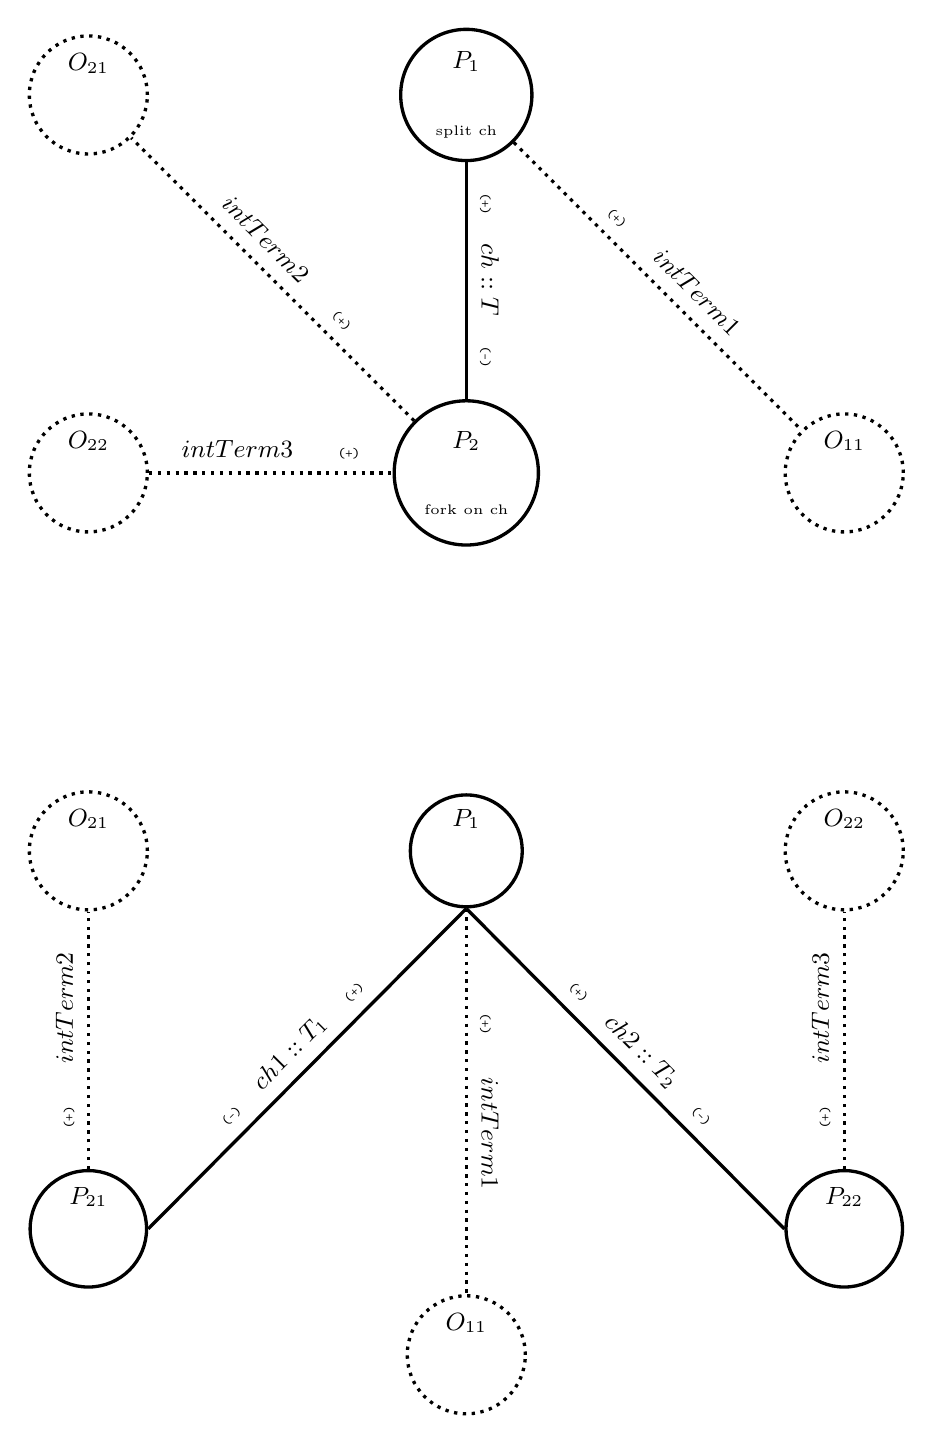
\begin{tikzpicture}[scale = .8,every node/.style={very thick}]
 \draw (6,0)  node[circle,draw=black,minimum size=0.4cm,align=center] (FP1)
              {\proc{P_{1}}{split ch}
              };

 \draw (0,0)  node[circle,draw=black,minimum size=0.1cm,align=center,dotted] (O21)
              {\proc{O_{21}}{}
              };

 \draw (0,-12)  node[circle,draw=black,minimum size=0.1cm,align=center,dotted] (SO21)
              {\proc{O_{21}}{}
              };

 \draw (0,-6)  node[circle,draw=black,minimum size=0.1cm,align=center,dotted] (O22)
              {\proc{O_{22}}{}
              };

 \draw (12,-12)  node[circle,draw=black,minimum size=0.1cm,align=center,dotted] (SO22)
              {\proc{O_{22}}{}
              };


 \draw (12,-6)  node[circle,draw=black,minimum size=0.1cm,align=center,dotted] (O11)
              {\proc{O_{11}}{}
              };


 \draw (6,-6)  node[circle,draw=black,minimum size=0.4cm,align=center] (FP2) 
              {\proc{P_2} {fork on ch}
              };


 \draw (6,-12)  node[circle,draw=black,minimum size=0.4cm,align=center] (SP1) 
              {\proc{P_1} {}
              };

 \draw (0,-18)  node[circle,draw=black,minimum size=0.4cm,align=center] (P21)
              {\proc{P_{21}}{}
              };

 \draw (12,-18)  node[circle,draw=black,minimum size=0.4cm,align=center] (P22)
              {\proc{P_{22}}{}
              };

 \draw (6,-20)  node[circle,draw=black,minimum size=0.4cm,align=center,dotted] (SO11)
              {\proc{O_{11}}{}
              };

 \draw[-,draw=black,very thick] (SP1.south) -- (P21.east) 
    node[midway,above=1pt,sloped,fill=white]   {\rlab{ch1::T_1}};
 \draw[-,draw=black,very thick] (SP1.south) -- (P22.west) 
    node[midway,above=1pt,sloped,fill=white]   {\llab{ch2::T_2}};
 \draw[-,draw=black,very thick] (FP1.south) -- (FP2.north) 
    node[midway,above=1pt,sloped,fill=white]   {\llab{ch::T}};

 \draw[-,draw=black,very thick,dotted] (O22.east) -- (FP2.west) 
    node[midway,above=1pt,sloped,fill=white]   {\rplab{intTerm3}};

 \draw[-,draw=black,very thick,dotted] (FP2.north west) -- (O21.south east) 
    node[midway,above=1pt,sloped,fill=white]   {\rplab{intTerm2}};

 \draw[-,draw=black,very thick,dotted] (FP1.south east) -- (O11.north west) 
    node[midway,above=1pt,sloped,fill=white]   {\plab{intTerm1}};

 \draw[-,draw=black,very thick,dotted] (SP1.south) -- (SO11.north) 
    node[midway,above=1pt,sloped,fill=white]   {\plab{intTerm1}};

 \draw[-,draw=black,very thick,dotted] (P21.north) -- (SO21.south) 
    node[midway,above=1pt,sloped,fill=white]   {\plab{intTerm2}} ;

 \draw[-,draw=black,very thick,dotted] (P22.north) -- (SO22.south) 
    node[midway,above=1pt,sloped,fill=white]   {\plab{intTerm3}} ;


\end{tikzpicture}
\end{center}
\caption{{\sf split-Fork} Example  $~(T~=~T_1 \oplus T_2)$} 
\label{fig:Conc_sfork_exam}
\end{figure}

\subsection {close-halt Constructs}\label{conc:haltclosedesc}
Before closing an MPL process, it is required to close all the channels associated with that process. {\sf close-halt} constructs are used to close a channel. By convention all the channels except the last channel are {\sf closed}. The last channel is {\sf halted} signifying the halting of the process.

\end {document}

